  \documentclass[journal,12pt,twocolumn]{article}
\usepackage{blindtext}
\usepackage{graphicx}
\graphicspath{{./figs/}}
\usepackage{amsmath,amssymb,amsfonts,amsthm}
\usepackage{watermark}
\newcommand{\myvec}[1]{\ensuremath{\begin{pmatrix}#1\end{pmatrix}}}

\let\vec\mathbf
\thiswatermark{\centering \put(-20,-55){
\includegraphics[scale=0.5]{iith.png}} }
\begin{document}
\title
{Optimization}
\author{mohammad imran}

\maketitle
\tableofcontents
\bigskip
\section{Problem Statement}
On the interval [0,1] the function $x^{25}(1-x)^{75}$ takes its maximum value at point ?\\
%\section{Construction}
%\begin{figure}[h]
%    \centering
%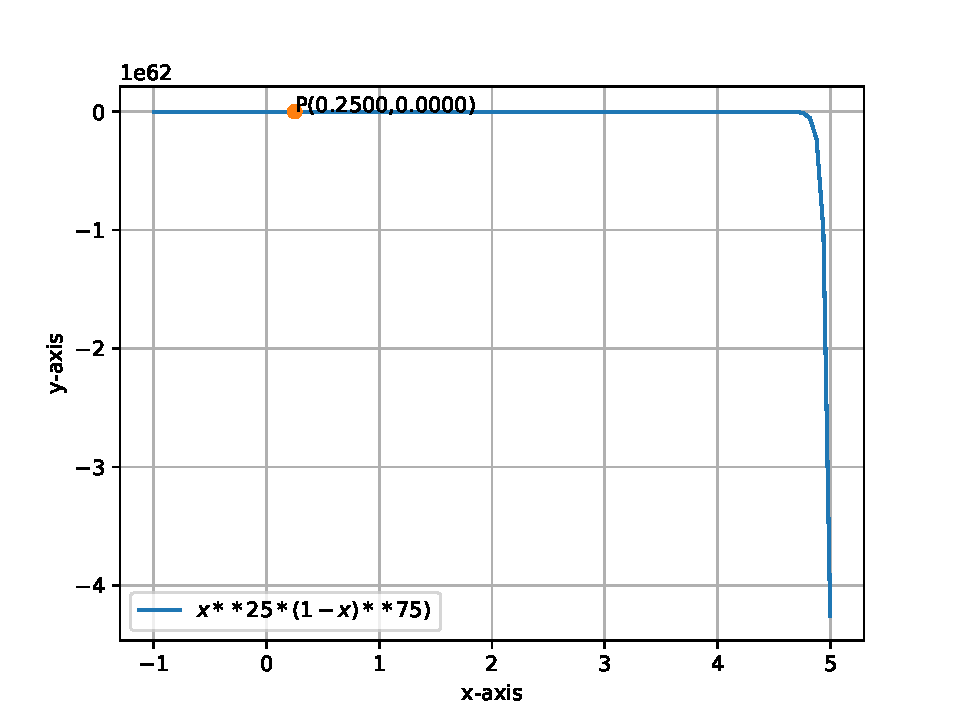
\includegraphics[width=\columnwidth]{fig.pdf}
%    \caption{using gradient ascent method}
%   \label{fig:my_label}
%\end{figure}


\section{Solution}
Given, \\
\\f(x)=$x^{25}(1-x)^{75}$\\

$f'(x)=25x^{24}(1-x)^{74}(1-4x)$\\
\\
\\we have to obtain the maximum value of $x^{25}(1-x)^{75}$ in the interval [0,1].this can be seen figure f(x).\\
\vspace{0.3cm}\\
\textbf{objective function:}
\begin{align}
f(x)= \max_\vec{x}(x^{25}(1-x)^{75})\\
\end{align}

\textbf{constraints}
\begin{align}
0<x<1
\end{align}
\\using \textbf{gradient ascent} method we can find its maxima in the interval [0,1].
\vspace{0.5cm}
\begin{equation}
 x_{n+1} = x_n + \alpha \nabla f(x_n)
\end{equation}
\vspace{0.2cm}
\begin{equation}
\implies x_{n+1}=x_n+\alpha(25x^{24}(1-x)^{74}(1-4x))
\end{equation}
\vspace{0.5cm}

Taking $x_0=0.25\alpha=0.001$ and precision = 0.00000001, values obtained using python are:
    

    \begin{align}
        \boxed{\text{Maxima} = 3.785253}\\
        \boxed{\text{Maxima Point} = 0.25}
    \end{align}\\
    
   \section{Construction}
\begin{figure}[h]
    \centering
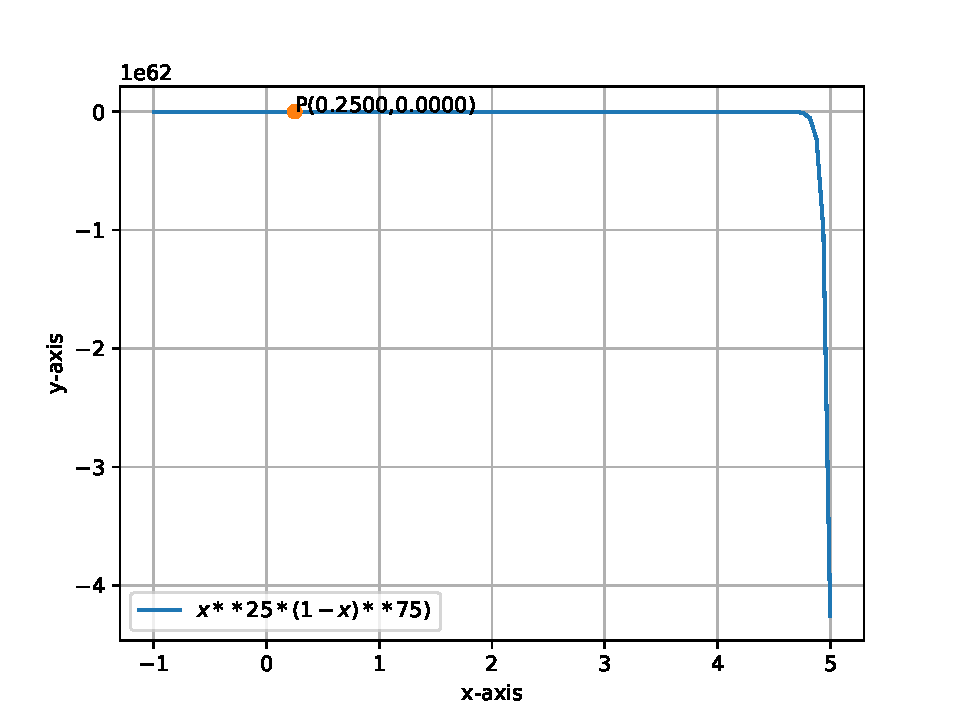
\includegraphics[width=\columnwidth]{fig.pdf}
    \caption{using gradient ascent method}
   \label{fig:my_label}
\end{figure}

    
\section{Software}
Download the following code using,
\begin{table}[h]
    \centering
    \begin{tabular}{|c|}
    \hline \\
        https://github.com/imran111888/fwc2/tree/main/optimization assignment\\
         \\
\hline
    \end{tabular}
\end{table}
\\
and execute the code by using command
\begin{center}
\textbf{Python3  opt.py}\\
\end{center}

\section{Conclusion}
We found the maxima and maximum value at the point .

\end{document}